\documentclass{article}
\usepackage{graphicx}
\usepackage{xcolor}
\usepackage{subcaption}
\usepackage[margin=1.0in]{geometry}

\begin{document}
\section{Introduction}
\begin{enumerate}
\item \textbf{General goal: }
Systematically develop model Hamiltonians which can accurately describe the energies as well as one- and two-particle properties of the lowest lying eigenstates for transition-metal oxide (TMO) molecules.

\item \textbf{Barrier to achieving that goal: } The necessity for many-body interactions in describing the low-lying excited states of TMO molecules poses a difficult challenge when developing model Hamiltonians.

\item \textbf{State of the art: } Common approaches to building these model Hamiltonians use effective single particle theories like Density Functional Theory (DFT) to generate an effective 1-body model or use the known energy spectrum of the TMO molecules to fit a model with many-body interactions. 
\textcolor{red}{Have to find references for this one, not sure how true this is.}

\item\textbf{How are we advancing state of the art: } We have systematically developed a many-body model which can accurately describe the energies, one- and two-particle properties of the lowest lying eigenstates for the neutral CuO molecule using \textit{ab-initio} Quantum Monte Carlo (QMC) calculations and a density-matrix downfolding (DMD) procedure. 
\end{enumerate}

\section{Figures}

%Figure 1
\begin{figure}
\centering
\begin{subfigure}{.5\textwidth}
  \centering
  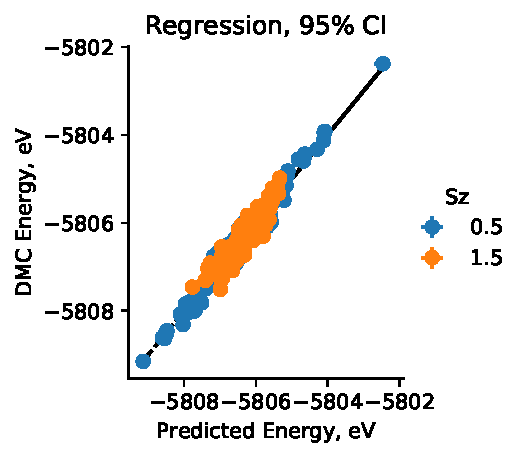
\includegraphics[width=\linewidth]{../qwalk/ub3lyp_s1_/analysis/fit_0_sel2_log.pdf}
  \caption{Prediction of linear regression on full set of samples.}
  \label{fig:Regression1}
\end{subfigure}%
\begin{subfigure}{.5\textwidth}
  \centering
  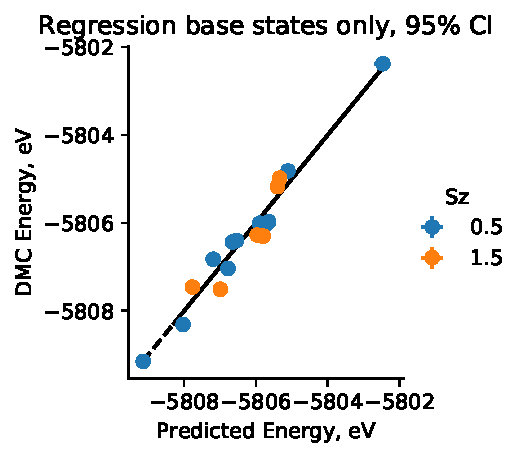
\includegraphics[width=\linewidth]{../qwalk/ub3lyp_s1_/analysis/fit_0_sel2_log_base.pdf}
  \caption{Prediction of linear regression on base states only.}
  \label{fig:Regression2}
\end{subfigure}
\label{fig:Regression}
\caption{Linear regression predictions for total energy compared to DMC energies.}
\end{figure}

%Figure 2
\begin{figure}
\centering
\includegraphics[width=\linewidth]{../qwalk/ub3lyp_s1_/analysis/}
\label{fig:Regression}
\caption{Results for energies and 1-/2-body properties of eigenstates from exact diagonalization of our model Hamiltonian.}
\end{figure}

\section{Supplementary Material} 

\end{document}